
\section{Brief overview of the domain} \label{sec:domain-overview}

The purpose of memory profilers is capturing information regarding how applications use memory.
However, to define memory profilers, a clear understanding about their nature is required.
Informally, the term \textit{memory profiling} refers to any kind of \textbf{\textit{process to collect}} some \textbf{\textit{data about the memory usage}}.
In an object-oriented runtime environment such as Java, such data may be as simple as the number of objects of a specific class, but it may also be as complex as the list of possible memory leak's sources.
Some other examples include computing the number of objects reachable from a specific class object; finding out if there is an instance of class $A$ which is referencing an object of class $B$; and computing, for each \textit{String}, its length and the number of objects that make direct reference to the \textit{string}.
The data collected by a profiler may have an arbitrary complexity; it may be a simple natural number, a boolean value, a list of values, or a composed value.
For instance, an integer value is required to describe one of the aforementioned examples, the number of objects reachable from a specific class object.
In the same way, a pair $\langle l,r \rangle$, where both $l$ and $r$ are integers, is required to store the result of determining for a \textit{string}, its length and the number of objects referencing it.
%The data collected by a profiler may have an arbitrary complexity

%The rest of this section introduces the vocabulary we use in the domain of memory profilers.

Formally, we use a set of concepts that is useful to properly define our understanding of the term profiler, and how we address their construction in this chapter.
The following concepts are used int the rest of the chapter:

\begin{description}
\item[Object] is an atomic entity that consumes memory to store the value of its attributes.
When we say \textit{object} we mean as in \gls{OOP}.
The operations that we can perform on these objects are nevertheless restricted to accessing attributes, obtaining the amount of memory used to represent an object, and accessing meta-data such as the class name.
Reusing the concept is ``natural'' since we are targeting MRTEs, which often support the object-oriented paradigm.

\item[Memory Heap] As mentioned this is the region of memory used to store dynamically allocated \textit{objects} that are connected through references forming a directed-acyclic graph.
It is also the universe $\mathbb{U}$ of objects.

\item[Structure] is a subset of \textit{objects} in the \textit{memory heap}.
The objects in an structure don't need to be directly related by references; instead, they can be arbitrarily composed.
For instance, the smallest non-empty \textit{structure} we can consider, is a structure containing a single object.
Only one property is required in properly formed structures;  $S_1 \bigcap S_2 = \emptyset$ for any pair of structures $S_1$ and $S_2$, which means that they are disjoint sets.

\item[Memory Profile] is a value that can be computed using information from the \textit{objects} (and their references) included in a \textit{structure}.
An example of useful value is the total size of a structure, which can be easily calculated using the function $\textit{total\_size}\left(S\right) = \sum_{o \in S} {sizeof(o)}$.
A common pattern of use is to identify many \textit{structures} in the heap, and then to compute a value -- not necessarily the same -- for each structure.

\item[Memory Profiling] consists in identifying \textit{structures}, and computing some values associated to these structures. 

\item[Structure types] provide a mean to describe several structures using a single pattern.
In other words, many time the heap can be partitioned in different structures, but it is hard to manually enumerate them.
The point is that we need a procedural way to describe what structures exist, and what are their membership functions; \textit{structure types} provide such facilities.
In particular, they provide (i) functions to evaluate whether an object is member of a \textit{structure}, (ii) ways to define the values corresponding to the \textit{memory profile} of a \textit{structure}, and (iii) factories to identify all \textit{structures} in the \textit{memory heap}.

\end{description}

%\extracomment{TODO}{Add example of structures in a graph, all connected to the fact that roots are in threads}

\paragraph{Objects reachable from a specific class object}

\begin{figure}[!ht]
\centering
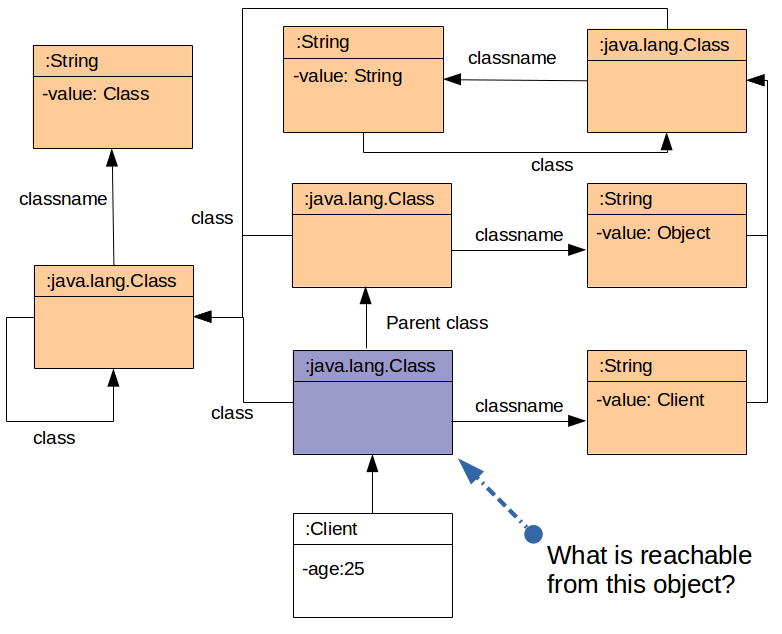
\includegraphics[scale=0.5]{./chapter6/fig/example1.png}
\caption{Objects reachable from the Client class. Observe that only one object is not reachable.}\label{fig:reachable-from-class-object}
\end{figure}

Mostrar la necesidad de atravesar el grafo para calcular la informacion

\paragraph{Is there an instance of A making reference to an object of type B?}

\paragraph{Length of each string, and number of objects referencing each string}

\paragraph{Length of each linked list}

Mostrar como hay patrones similares que se pueden detectar muchos

\begin{figure}[!ht]
\centering
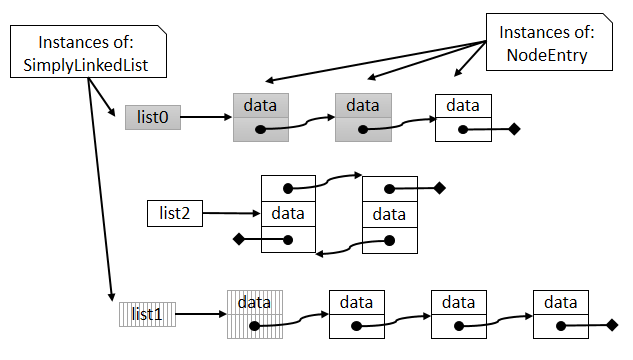
\includegraphics[width=0.65\linewidth]{chapter6/fig/lists}
\caption{Memory snapshot with three linked lists}
\label{fig:simple_snapshot}
\end{figure}


\section{Metalanguage to define custom memory profilers}\label{sec:approach}

In this chapter, we propose a tool to create custom memory profilers for MRTEs.
We are interested on easing the task of defining new profilers without sacrificing their performance regarding CPU consumption.
Keeping the profiler's overhead as low as possible is of utmost importance for us because lightweight profilers can be use both during the development phase and during the application execution in a production environment.
To reach this goal, we propose a Domain Specific Language (DSL) and its code generator which aims at describing and generating efficient online memory profilers. 

We next present the syntax, semantics and usage examples of our domain-specific language.

\subsection{Abstract Syntax}\label{sec:abstract-syntax}

The metamodel shown in Figure~\ref{fig:as} describes the abstract syntax of our DSL.
The main concept of this metamodel is a \textit{CustomProfiler} which is composed of \textit{UserDefined} types and a \textit{StructureFactory}.
The concepts related to \textit{UserDefined} types are shown on the left part of the metamodel, while the right part describes the \textit{StructureFactory} which represents both the set of  structures to identify and the value to compute on these structures.

\subsubsection{User-defined types}
In addition to various \textit{BasicTypes} such as \textit{Integer}, \textit{String} and \textit{Boolean}, the language supports the definition of both \textit{Records} and \textit{Lists}.
As expected, a \textit{record} contains \textit{fields} to hold values of previously defined types.
Likewise, a \textit{list} refer to a \textit{base type}; hence all the members of a list must be of the same type.
In a custom profiler, \textit{UserDefined} types can be composed in arbitrary ways as long as no type contains a recursive declaration.
We can formalize such a constrain using OCL (Object Constraint Language~\footnote{\url{http://www.omg.org/spec/OCL/}}):

\begin{lstlisting}[escapeinside={(*}{*)},
label=fig:membership,
language=OCL1
]
context Record inv: 
   not fields->oclAsSet()->closure(t)->exists(t | t = self)

context List inv:
   not baseType->oclAsSet()->closure(t)->exists(t | t = self)
\end{lstlisting} 

A \textit{List} has operations to manipulate any value which represent a list.
Figure~\ref{fig:as} shows a subset of these operations.
In general, these operations correspond to the set of \textit{standard} operations of any implementation of the list data type.

\subsubsection{Defining structures to profile}
Defining the \textit{StructureFactory} is the core of writing a custom profiler.
A \textit{StructureFactory} contains an \textit{Expression} through the \textit{instances} relationship which indicates a pattern to identify structures in the memory heap.
Notice that a single instance of \textit{StructureFactory} creates many data structures in memory; thus the \textit{Expression} corresponds to a list indicating that a new structure must be instantiated for each element of the list.
Forcing the \textit{Expression} to be a \textit{List} can be easily formalized using OCL:

\begin{lstlisting}[escapeinside={(*}{*)}, label=fig:instances, language=OCL1]
context StructureFactory inv: instances.type.oclIsTypeOf(List)
\end{lstlisting}

Defining a new \textit{StructureFactory} implies defining its \textit{type} which is an instance of \textit{StructureType}.
This concept describes the mechanism used to populate, out of objects, a structure and its information.
In short, each structure in memory instanciated through a \textit{StructureFactory} has a type \textit{StructureType}.
For example, we may be interested in finding all the \textit{SimplyLinkedList} in the memory snapshot depicted in Figure~\ref{fig:simple_snapshot}.
In such a case, there are two \textit{SimplyLinkedList}, but we only need one mechanism to identify them because they have the same pattern in memory. 

\begin{figure*}
\centering
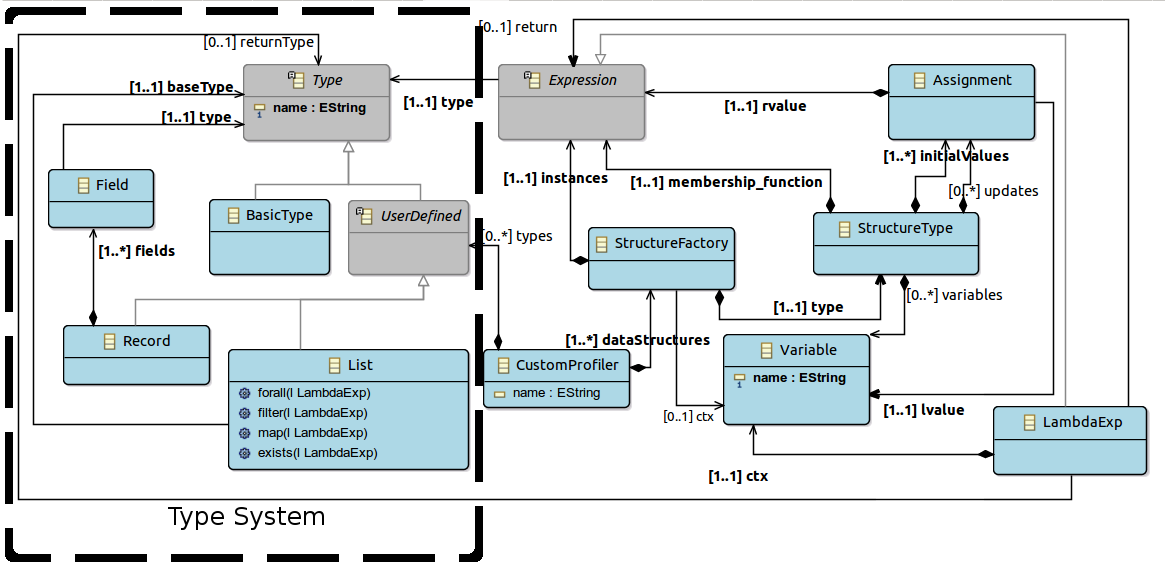
\includegraphics[width=0.87\linewidth]{chapter6/fig/AS}
\caption{Custom profiler Metamodel}
\label{fig:as}
\end{figure*}


A \textit{StructureType} is composed of \textit{Assignments} that are used as \textit{initialValues} for each \textit{Variable} holding information - similar to a constructor in object-oriented programming.
Once a new structure is created, the \textit{Assignments} are executed to assign the initial value of each \textit{Variable}.
Observe that \textit{variables} do not refer to a \textit{Type}.
Our DSL is strongly typed and the \textit{type} of each user-defined variable is inferred from its initial value.
Nevertheless, there is a built-in variable in each \textit{StructureType} that is only accessible during initialization.
Its type is predetermined as part of the language specification.
We force the use of the proper type using OCL:

\begin{lstlisting}[escapeinside={(*}{*)}, label=fig:instances, language=OCL1]
context StructureType inv:  initialValues->exists(a: Assignment | 
     a.lvalue.name = 'initialObjects' and a.rvalue.type.oclIsTypeOf(List)
   ) 
\end{lstlisting}

In addition, a \textit{StructureType} contains a boolean \textit{expression} which is the \textit{membership function} used to decide whether an object should be included in the structure instance.
Finally, it also contains a set of \textit{Assignments} to update the value of each \textit{variable} every time a new object is included in the structure.
This set of \textit{Assignments} is used to compute the actual value of the memory profile.
The major constraint regarding these \textit{updates} is that they must refer to already initialized \textit{variables} and the new assigned values must match the previous types.
We formalize such a constrain using OCL:

\begin{lstlisting}[escapeinside={(*}{*)}, label=fig:lvalue, language=OCL1]
context StructureType inv:  updates->forAll(a: Assignament | 
    self.initialValues->exists(aa : Assignament | 
       aa.lvalue = a.lvalue and aa.rvalue.type = a.rvalue.type
     ))
\end{lstlisting}

In our DSL, \textit{expressions} play a big role.
For the sake of readability, Figure~\ref{fig:as} only shows a couple of concepts related to them.
However, it is noteworthy that, in addition to \textit{arithmetic}, \textit{boolean} and \textit{literals} for basic types, the language includes lambda expressions, literal for records and lists.
Moreover, the language defines \textit{built-in rvalues} which are nothing but expressions initialized by the runtime within a specific scope.
Instead of being user-defined, the types of these expressions are also defined by the runtime.
There are two types of \textit{built-in rvalues}, target independent and dependent.
Among the firsts, we have the list of  \textit{objects}, a reference to the \textit{current data structure} and a reference to the \textit{current object}.
Target dependent \textit{rvalues} in Java include the list of \textit{loaded classes} and the list of \textit{threads}.
The precise meaning of these \textit{rvalues} as well as their scopes are precisely discussed in sections~\ref{sec:concrete-syntax}, ~\ref{sec:semantic} and~\ref{sec:implementation} along the concrete syntax, the language semantic and the tooling support.

Finally, if we use the memory snapshot depicted in Figure~\ref{fig:simple_snapshot}, calculating the number of nodes belonging to a specific \textit{SimplyLinkedList} is an example that illustrates the language's concepts.
To solve this problem we can instantiate the metamodel of our DSL as follow:
\begin{itemize}
\item Define a \textit{StructureFactory} in which the \textit{instances} property is a list which contains the objects \textit{list0} and \textit{list1}.
\item Instantiate a \textit{StructureType} where the built-in variable \textit{initialObjects} receives as value a list with one member - list0 or list1.
      The other properties of this \textit{StructureType} instance are detailed in the next steps: 
      \begin{enumerate}
      \item Define a variable \textit{n} with initial value zero.
      \item Define a membership function which return true if an object is instance of \textit{NodeEntry} and it is referenced by an object for which the membership function also return true. Observe how this recursive function returns true for each element in \textit{list0} because the initial object's list contains object \textit{list0}. 
      \item Update the variable \textit{n} by increasing its value by one.
      \end{enumerate}  
\end{itemize}
Further details about this example are discussed in the next section.

\subsection{Concrete Syntax}\label{sec:concrete-syntax}

A textual concrete syntax has been defined for our DSL allowing the domain expert to define a custom memory profiler using a text editor.
A high-level view of the grammar for this textual representation is depicted in Figure~\ref{fig:dsl-grammar}.
As can be seen, the rules that represent expressions make such a grammar ambiguous, we decided to use this form for the sake of the presentation.
However, a complete LL(*) grammar~\cite{Parr:2011:LFA:1993498.1993548} is presented hereafter in Annex~\ref{anx:grammar}.
One interesting aspect of this concrete language is its relative verbosity.
For instance, it uses very explicit keywords such as ``create structure foreach'', ``constructor'', and ``membership''.


%\setlength{\grammarparsep}{20pt plus 1pt minus 1pt}
{
\scriptsize
\begin{figure}[!ht]
\begin{mdframed}[outermargin=0.2cm, innermargin=0.5cm]

\newcommand{\grule}[1]{\hfill{\scriptsize (#1)}}
\setlength{\grammarindent}{5em}
\begin{grammar}

<program> ::= <types> <structures> \grule{1}

<types> ::= <type> <types> | <empty> \grule{2, 3}

<type> ::= <id> `:' `table-of' <id> | <id> `:' `struct' `{' <fields> `}' \grule{4, 5}

<fields> ::= <id> `:' <id> <fields> | <id> `:' <id> \grule{6, 7}

<structures> ::= <struct-factory> <structures> | <struct-factory> \grule{8, 9}

<struct-factory> ::= `create structure foreach' <id>`:'<e> `using' <body> \grule{10}

%<Header> ::= `create structure foreach' <id>`:'<expr>

<body> ::= `constructor' <s> `membership' <expr> `updates' <s> \grule{11}

%<constructor> ::=  \grule{12}

%<membership> ::= 

%<updates> ::= \grule{13}

<s> ::= <a> <s> | <empty> \grule{12}

<a> ::= <id> `=' <e>  \grule{13} 

<e> ::= <e> <binary-op> <e> | <unary-op> <e> \grule{14, 15}
\alt <e> `in' <id> | <e> `is' <id> \grule{16, 17}
\alt <e> `.' <id> `(' <expr-list> `)' \grule{18}
%\alt <e> `.' <id> `(' `[' <id> `|' <s> `]' `)' \grule{19}
\alt <e> `.' <id>                              \grule{20}
\alt `#[' <expr-list> `]' | `struct' <id> `{' <expr-list> `}' \grule{21, 22}
\alt <int-literal> | <string-literal> | <bool-literal> \grule{23, 24, 25}
\alt <id> | `(' <e> `)' \grule{26, 27}

<expr-list> ::= <e> `,' <expr-list> | `[' <id> `|' <s> `]' `,' <expr-list> | <empty>  \grule{28}

<binary-op> ::= `+' | `*' | `-' | `/' | `and' | `or'

<unary-op> ::= `-' | `not'

\end{grammar}
\end{mdframed}
\caption{Concrete grammar of the language. For the sake of clarity, we are using an ambiguous grammar to describe the expression language.} \label{fig:dsl-grammar}
\end{figure}
}

As an example, the next listing shows how to compute the length of each \textit{SimplyLinkedList} in the memory snapshot depicted in Figure~\ref{fig:simple_snapshot}.
The mechanism is based on counting the number of \textit{NodeEntry} referenced by the \textit{SimplyLinkedList}.
Each \textit{NodeEntry} is used to wrap one element of data and to point to the next element.

\begin{lstlisting}[escapeinside={(*}{*)}, 
label=lst:listLengt, language=DSL2
]
create structure foreach e:objects.filter(l| l is SimplyLinkedList) using
  constructor
    initialObjects = #[e] // a list literal with one element: e
    n = 0
  membership (this is NodeEntry) and (referrer in this_structure)
  updates 
    n = n + 1
\end{lstlisting}

In the example, only one \textit{StructureFactory} is necessary.
In line 1, we define the list of structures we are interested in.
We do so by selecting instances of class \textit{SimplyLinkedList} as elements of the \textit{StructureFactory}.
Since there are two simply linked lists in the memory snapshot, we are going to build two structures.
Observe the usage of a built-in \textit{rvalue} named \textit{objects} which contains all the objects in memory.
The valid scope of this rvalue is in both the definition of the set of structures and the computation of the initial values.
Thereafter, lines 2-4 specify the initial values.
Line 3 in particular initializes the set of objects included in the structure.
Notice the usage of a list literal to include the object referenced by \textit{e}.
In the initialization scope, the rvalue \textit{e} is equal to one of the element within the list of structures - either \textit{list0} or \textit{list1}.

In line 5 we define the membership function, which is used to determine if an object is part of the structure.
There are four built-in rvalues during the evaluation of the function as well as during the update of the variables.
First, the value named \textit{this} is the current visited object. 
The \textit{membership} boolean \textit{expression} aims at determining if this object is part of the \textit{structure} or not. 
The value \textit{this\_structure} identifies the structure.
As our runtime profiler will traverse the graph of in memory objects following references between objects, the object through which we have reached the \textit{this} object is known as \textit{referrer}.
The last value, which is target dependent, is the kind of reference.
Operator \textbf{is} checks if \textit{this} is an instance of class \textit{NodeEntry}.
Likewise, operator \textbf{in} checks whether the \textit{referrer} is already a member of the structure.
Finally, line 7 updates the length of the list when an object is detected as member of the structure.

\subsection{Operational Semantics}

\extracomment{TODO}{
\begin{enumerate}
\item Add notation
\item Fix the rule that calls a method with a lambda expression
\item Add the rule for the interpretation of a program
\item Discuss the inference rules
\end{enumerate}
}

\begin{figure}
\begin{mdframed}[innermargin=0.3cm, outermargin=0.3cm]

{
\footnotesize

\begin{tabular}{rcl}
$Bool(1)$ and $Bool(0)$ & & \parbox{8cm}{Values  $true$ and $false$.}\\
& & \\
$ E $ & \parbox[t]{0.7cm}{} & \parbox{8cm}{Describes a mapping from \textit{identifiers} to \textit{locations}. We use $id \mapsto l$ to represent a member of the mapping} \\ 
& & \\
$ S $ & & \parbox[t]{8cm}{Describes a mapping from \textit{locations} to \textit{values}. Informally, it can be seen as the storage. We use $l \mapsto v$ to represent a member of the a mapping.} \\ 
& &  \\
$ C $ & & \parbox[t]{8cm}{Describes a mapping from \textit{values} to \textit{structures}. We use $v \mapsto s$ to represent a member of the mapping.} \\ 
& & \\
$\left[ k_1 \mapsto v_2, \dots, k_n \mapsto v_n \right]$ & & \parbox[t]{8cm}{Describes a mapping by enumerating its members.} \\ 
& & \\
$S\left[ v_i/k_i \right]$ & & \parbox[t]{8cm}{Describes a new mapping where $S\left[ v_i/k_i \right](k_j) = S(k_j)$ if $k_i \ne k_j $, $S\left[ v_i/k_i \right](k_j) = v_i$ otherwise. } \\
& &  \\
$M \overset{\operatorname{val\_of}}{\vdash} k \mapsto v$ & & \parbox[t]{8cm}{A set of auxiliary rules to compute the value $v$ that is associated to the key $k$ in the mapping $M$.} \\ 
& &  \\
$C \overset{\operatorname{contains}}{\vdash} v \mapsto s \Rightarrow r$ & & \parbox[t]{8cm}{A set of auxiliary rules to determine whether the value of $v$ is mapped to $s$ in $C$, which is always a mapping from  \textit{values} to \textit{structures}. $r$ is a boolean value. } \\
& &  \\
$\lVert E,S, id, e\rVert$ & & \parbox[t]{8cm}{Describe a closure, $E,S$ represents the state, $id$ is the identifier used as parameter of the closure, and $e$ is the expression to evaluate.} \\ 
& & \\
$T(a_1 \mapsto l_1, \dots, a_n \mapsto l_n)$ & & \parbox[t]{8cm}{A generic value in the language. $T$ is its type, and a mapping from attributes $a_i$ to their respective locations $l_i$. Sometime, we use $\mathbb{A}$ to represent the mapping. There are shorthands for special cases: $Bool(1)$, $Bool(0)$, $Int(n)$ which is the integer $n$, and $String(w)$ which is the string $w$. In addition, the value $table(l_1,\dots,l_n)$ denotes a table; in this case, $l_i$ is the location in storage of the \textit{i-th} element of the table. } \\ 
& & \\
$\langle T, P, a_1 \mapsto T_1, \dots, a_n \mapsto T_n \rangle$ & & \parbox[t]{8cm}{Describe a type with identifier $T$. The description contains the parent type $P$ (which has the same structure), and its attributes $a_i \mapsto T_i$. } \\
& & \\ 
$\overset{\operatorname{subtype}}{\vdash} S, P \Rightarrow r$ & & \parbox[t]{8cm}{A set of auxiliaries rules to determine whether type $S$ is a subtype of $P$. $r$ is a boolean value.} 
\end{tabular} 

}

\end{mdframed}
\caption{Notation used in the operational semantic}\label{fig:notation-for-operational-semantic}
\end{figure}

\renewcommand{\inference}[3][]{%
  \begin{array}[b]{@{}c@{}c@{}}
    \smash{\raisebox{-.5\normalbaselineskip}{{\scriptsize #1}}} & 
      \begin{array}[b]{l}
        #2
      \end{array} \\
      \cline{2-2}
    & \begin{array}[t]{c}
        #3
      \end{array}
  \end{array}
}

\mathlig{->}{\mapsto}
\mathlig{|-}{\vdash}
\mathlig{=>}{\Rightarrow}
\mathlig{"}{\;\;\;}

\mathligson

% classics
{
\footnotesize
\[
% true
\textnormal{{\scriptsize It(25):}}\; E, S\vdash\operatorname{true}\Rightarrow Bool(1),S
\quad\quad
% false
\textnormal{{\scriptsize It(25):}}\; E, S\vdash\operatorname{false}\Rightarrow Bool(0),S
\]

\[
% integers
\textnormal{{\scriptsize It(23):}}\; E, S\vdash\operatorname{Integer}\; N\Rightarrow Int(N),S
\quad\quad
% strings
\textnormal{{\scriptsize It(24):}}\; E, S\vdash\operatorname{String}\; w\Rightarrow String(w),S
\]

% lambda expressions
\[
\textnormal{{\scriptsize It(19):}}\; E, S\vdash \left[id \vert e \right] \Rightarrow \lVert E,S, id, e\rVert,S
\]

\[
% id
\inference[It(26):]{
E\overset{val\_of}{|-}id->l_{id} "" S\overset{val\_of}{|-}l_{id}->v
%v = S \; E \; id
}{E, S|-id=>v,S}
\quad\quad
% (e) 
\inference[It(27):]{
E, S|-e=>v,S_1
}
{E, S|-(e)=>v,S_1}
\]

\[
% unary operators
\inference[It(17b):]{
E, S|-e_0=>v_0,S_1
}{E, S|-\operatorname{op}e_0=>\operatorname{op}v_0,S_1}
\quad\quad
% binary operators
\inference[It(17a):]{
E, S|-e_0=>v_0,S_1 "" E, S_1|-e_1=>v_1,S_2
}{E, S|-e_0\operatorname{op}e_1=>v_0\operatorname{op}v_1,S_2}
\]

\[
% in operator
\inference[It(17c):]{
C, E, S|-e_0=>v_0,S_1 "" C \overset {in} {|-} v_0->id =>v
%v = v_0->id \in C? Bool(1):Bool(0)
}{C, E, S|-e_0 \; in \; id=>v,S_1}
\quad\quad
\]

\[
% is operators
\inference[It(17d):]{
E, S|-e_0=>X(\mathbb{A}),S_1 "" \overset{subtype}{|-} X, T \Rightarrow v
}{E, S|-e_0\; \operatorname{is} \; T:v,S_1}
\]

\[
% assignment
\inference[It(16):]
{
E,S|-e_0=>v_0,S_1 "" E\overset{val\_of}{|-}id->l_{id}
%l_{id} = E(id) \\
%S_2 = 
}
{E, S|-id = e_0=>v_0, S_1[v_0/l_{id}]}
\quad\quad
% statements
\inference[It(14)]
{
E, S|-a=>v_a,S_1 "" E, S_1|-s=>v,S_2
}
{E, S|-a\;s=>v,S_2}
\]

\[
% struct literal
\inference[It(22):]
{
E,S|-e_1:v_1,S_1 \\
\vdots \\
E,S_{n-1}|-e_n:v_n,S_n \\
\operatorname{class}(T)=(a_1->T_1, \dots, a_n->T_n) \\  % take the fields of the object
l_i = \operatorname{newloc}(S_n) \; for \; i = 1 \dots n \\
v=T(a_1->l_1, \dots, a_n->l_n) \\ % assign locations to fields
S_f = S_n[v_1/l_1, \dots, v_n/l_n]
}
{E, S|-struct\;T\;\{ e_1, \ldots, e_n \}:v,S_f}
\quad\quad
% list literal
\inference[It(21):]
{
E,S|-e_1:v_1,S_1 \\
\quad \vdots \\
E,S_{n-1}|-e_n:v_n,S_n \\
l_i = \operatorname{newloc}(S_n) \; for \; i = 1 \dots n \\
v=\operatorname{Table}(l_1, \dots, l_n) \\
S_f = S_n[v_1/l_1, \dots, v_n/l_n]
}
{E, S|-\#[e_1, \dots, e_n]:v,S_f}
\]

\[
% accessing field
\inference[It(20):]{
E,S|-e=>X(\mathbb{A}),S_f "" \mathbb{A} \overset{val\_of}{|-} \textit{id} -> l_{\textit{id}} "" \mathbb{S} \overset{val\_of}{|-} l_{\textit{id}} -> v
%v0 = X(a_1->l_1, \dots, a_n->l_n) \\
%l_{id} = l_i \; where \; a_i = id \\
%v = S_1(l_{\textit{id}}) \\
}
{E,S|-e.\textit{id}=>v,S_f}
\]

\[
% calling method
\inference[It(18):]{
E,S|-e_0=>X(\mathbb{A}),S_0 \\
E,S_0|-e_1=>v_1,S_1 \\
""" \vdots \\
E,S_{n-1}|-e_n=>v_n,S_n \\
\operatorname{impl}(X,f) = (x_1, \dots, x_n, f_{body}) \\
l_{x_i} = \operatorname{newloc}(S_{n+1}) \; for \; i = 1 \dots n \\
\mathbb{A}[l_{x_1}/x_1, \dots, l_{x_n}/x_n],S_n[v_1/l_{x_1}, \dots, v_n/l_{x_n}]|-f_{body}:v,S_f
}
{E,S|-e_0.f(e_1, \dots, e_n):v,S_f}
\]

% news

%\[
%% lambda expressions
%\inference[It(19) mal]{
%v = \lVert E, \left[ id | s \right] \rVert " a " v
%}{
%E,S|-[id|s]:v,S
%}
%\quad\quad
%% calling function with lambda expression
%\inference[It(19) mal]{
%E,S|-e_0:v_0,S_1 \\
%v_0 = X(a_1=l_1, \dots, a_m=l_m) \\
%\operatorname{impl}(X,f) = (x_1, f_{body}) \\
%l_{x_1} = \operatorname{newloc}(S_1) \\
%E' = [a_1:l_1, \dots, a_m:l_m][l_{x_1}/x_1] \\
%v_1 = \operatorname{Clousure}(E, \left[ id | s \right]) \\
%v_0, E', S_1[v_1/l_{x_1}]|-f_{body}:v,S_f 
%}{
%E,S|-e_0.f\left( \left[ id | s \right] \right):v,S_f
%}
%\]
%
%}

\mathligsoff

\subsection{Translational Semantics}\label{sec:semantic}

An instance of our metamodel is compiled into a custom memory profiler.
This compilation produces a library written in \textit{C++} which is in charge of collecting the desired information from the runtime environment.
The generated source code has two parts.
First, for each \textit{StructureType} in the model, the compiler generates a subclass of \textit{AbstractStructureType} which is shown below.
Every subclass contains attributes to store the variables used in the associated \textit{StructureType}.
In the listing below, the class \textit{Context} holds the built-in values we mention in the previous section.
\begin{lstlisting}[language=C++, frame=L,
numbers=left,
numberstyle=\color{black}\scriptsize,xleftmargin=2\parindent]
class AbstractStructureType {
public:
	void initialize(Context& ctx) = 0;
	bool membership(Context& ctx) = 0;
	void update(Context& ctx) = 0;
}
\end{lstlisting}

The second part of the generated code is formed by a set of initialization routines, one for each \textit{StructureFactory}.
Each routine creates a list of structures with a specific \textit{AbstractStructureType} - the \textit{T} parameter in the listing.
Formally, the signature and behavior of these routines are as follow:
\begin{lstlisting}[language=C++, frame=L,
numbers=left,
numberstyle=\color{black}\scriptsize,xleftmargin=2\parindent]
template <typename T> void
[name](Context& ctx, std::vector<AbstractStructureType*>& s){
  for (Object obj : ctx.instances) {
    AbstractStructureType* ns = new T();
    ctx.e = obj;
    ns->initialize(ctx);
    s.add(ns); // not valid in the STL, but simpler to read
  }
}
\end{lstlisting}
An important concern during the transformation lies on efficiently mapping our concepts to \textit{C++} concepts.
Moreover, since each target platform provides facilities to get metadata regarding the objects in memory, using such facilities efficiently is specially important in order to reduce the performance overhead due to profiling.

The final profiler is built using both the generated code and a template algorithm.
The template is target dependent, but in general we use the underline target facilities to collect meta-data, access fields in certain steps, traverse the objects in memory and also to populate the built-in rvalues.
A simplified version of the used algorithm is shown below:
\begin{lstlisting}[escapeinside={(*}{*)},
label=lst:template, language=AlgLang, frame=L,
numbers=left,
numberstyle=\color{black}\scriptsize, xleftmargin=2\parindent]
values:
   structures: vector<AbstractStructureType*>
routine:
   foreach (initialization rountine (*$R_i$*) associated to a StructureFactory)
      create context
	  call (*$R_i$*)(context, structures)
   foreach (r: references among objects)
      if (r.target has no membership)
         create context // context.this = r.target
         S = structures.findfirst(s | s.membership(context))
         make context.this a member of S
         S.update(context)
   return structures 
\end{lstlisting}
There are two loops in the algorithm. 
The former loop is in charge of creating the set of structures the program is intended to collect information about.
The creation of the context in line 5 depends on the target platform.
It basically creates values such as the list of objects in memory or the list of loaded classes.
The latter loop traverses all the references among objects in memory.
During each iteration, the algorithm finds the first structure for which the membership function is true.
Notice that we only select the first because for some memory accounting problems, it is too hard to define a membership functions that build disjoints structures~\cite{dsn/09/geoffray/ijvm,Attouchi:2014:MMM:2602458.2602467}.
Thereafter, the information for such a structure is updated.

%The complete execution of a program in our language is as follow. Subgraph instances are initialized using listing~\ref{onInitialization}.
%Afterward, all the references in the graph of objects are traversed running listing~\ref{lst:onNodeFoundData}.
%The output data for all subgraph instances has been collected after all the references are traversed once.

%Finally, in listings~\ref{lst:onNodeFound},~\ref{lst:onNodeFoundData} and~\ref{onInitialization} we use built-in properties that are defined by the user.
%These properties must have access to some data describing the content of the memory in order to successfully identify subgraphs and calculate output values.
%Such data is wrapped in what we call execution context.
%In our DSL there are two different execution contexts: \textit{global context} and \textit{local context}.
%The former includes built-in values such as: i) lists of \textit{objects}, \textit{threads}, \textit{classes}, etc. , and ii) a value called \textit{Entity} representing a subgraph instance.
%The latter only contains the object \textit{THIS} which is being visited, a label of the reference representing its type, \textit{REFERRER} which is the object referencing the visited and again the \textit{Entity} value.
%The \textit{global context} is available in listing~\ref{onInitialization} while the \textit{local context} is available in both listings~\ref{lst:onNodeFound} and~\ref{lst:onNodeFoundData}.

\subsection{Language Usage}

\extracomment{FIX}{Improve explanations, add a caption to each listing, improve the style of each listing}

There are several possibilities for using our DSL in the various stage of an application lifecycle.
These include checking: local data structure invariants, reachability properties, memory consumption properties and combinations of those.
Below, we show some examples to highlight possible usage of our language. 
 
The first example shows how to assert the existence of a value satisfying some properties, independently of which object contains it. 
The result is obtained through the use of a filter on the list of objects.
The assertion successes if the heap contains an object with an attribute named $data$ with a value comprised between $3.141$ and $3.142$.

\begin{lstlisting}[escapeinside={(*}{*)},
%label=assertion, 
language=DSL2]
create structure foreach e:#["whole-jvm"] using
  constructor
    initialObjects = #[]
    existValue = false
  membership true
  updates 
    existValue = existValue or (this.data > 3.141 and this.data < 3.142)
\end{lstlisting}

The goal of next listing is to detect a bug identified in~\cite{Aftandilian:2009:GAU:1543135.1542503}.
This listing aims at finding if there exists an instance of the class $Order$
with the value of its field $field$ being equal to $specialValue$.
This technique is used to detect if one object has been garbage collected or if someone still holds a reference on it preventing its garbage collection.

\begin{lstlisting}[escapeinside={(*}{*)},
%caption=Detecting a knwon bug in pseudojbb., 
%label=pseudojbb,
%float=!h,
language=DSL2]
create structure foreach e:#["whole-jvm"] using
  constructor
	initialObjects = #[]
	fault = false
  membership  true
  updates
    fault = fault or (this is Order and this.field = specialValue)
\end{lstlisting}

The next example computes a combination of reachability and memory consumption properties.
It calculates the number of objects, and their total memory consumption, that are reachable from the threads.
We can notice how the membership property discards those objects that are not referenced by an already included object.  

\begin{lstlisting}[escapeinside={(*}{*)},
caption={Calculating objects reachables from threads},
label=kevoreeaccounting,
%float=!h,
language=DSL2]
create structure foreach e:#["whole-jvm"] using
  constructor
    initialObjects = threads
    nbObjects = 0 
    nbSize = 0 
  membership ( this in None and referrer in this_structure )
  updates 
    nbObjects = nbObjects + 1  
    nbSize = nbSize + this.size
\end{lstlisting}

We can also express complex structures in memory.
For instance, to find the consumption of K3-Al object namely \textit{K3Object} as described in Section~\ref{sec:chapter2-introduction}, we must find all instances of \textit{HashMap.Entry} that have \textit{K3Object} as the \textit{key}. These entries should be added to the consumption of the object \textit{K3Object} as well as all the objects reachable from the \textit{HashMap.Entry.value}.
To come out with this solution a good understanding of how K3-Al implements aspects is required.
The rationale here is that K3-Al stores the state of aspects in a separate HashMap, using as key the object to be aspectized.

\begin{lstlisting}[escapeinside={(*}{*)},
%caption=Computing the consumption of each K3-Al Object along with its aspects., 
%label=k3,
%float=!h, 
language=DSL2]
create structure foreach e:objects(*{.filter}*)([it|it is K3Object]) using
  constructor
    initialObjects = #[e]
    nbSize = 0
  membership (referrer in this_structure and this in None ) or
    (this is HashMap.Entry and this.key in this_structure and 
      this.key is K3Object)
  updates
    nbSize = nbSize + 1
\end{lstlisting}